% NP-Hardness Part 2 -- Metropolis beamer slides
% Compile: pdflatex np-hardness-part-2.tex (x2)
\documentclass[10pt,aspectratio=169]{beamer}

\usetheme{metropolis}
\metroset{block=fill, numbering=fraction, progressbar=frametitle}

\usepackage[T1]{fontenc}
\usepackage{amsmath, amssymb}
\usepackage{booktabs}
\usepackage{tikz}
\usetikzlibrary{arrows.meta, positioning, calc}

% ---- colors -------------------------------------------------------------
\definecolor{mLightBlue}{HTML}{4C72B0}
\definecolor{mGreen}{HTML}{55A868}
\definecolor{mRed}{HTML}{C44E52}
\definecolor{mGray}{HTML}{BFBFBF}
\definecolor{mOrange}{HTML}{DD8452}
\setbeamercolor{alerted text}{fg=mRed}

% ---- helpers ------------------------------------------------------------
\tikzset{
  lit/.style={draw, circle, minimum size=9mm, inner sep=0pt, font=\small,
              fill=white},
  pick/.style={lit, fill=mOrange!55},
  edg/.style={thick, mGray!80!black},
  conf/.style={thick, mRed!70, dashed},
  box/.style={draw, thick, rounded corners=3pt, minimum height=7mm,
              minimum width=22mm, align=center, font=\small},
  arr/.style={thick, -{Stealth[length=2.5mm]}},
  % overlay-aware keys: onslide=<2->{pick}
  onslide/.code args={<#1>#2}{\only<#1>{\pgfkeysalso{#2}}},
}

% ---- title --------------------------------------------------------------
\title{NP-Hardness, Part 2}
\subtitle{NP-Hard, NP-Complete, SAT, Cook-Levin, Reductions}
\date{}
\author{}

\begin{document}

\maketitle

% =========================================================================
\begin{frame}{Recap}
  \begin{itemize}
    \item $\mathbf{P}$: decision problems \alert{solvable} in polynomial
          time.
    \item $\mathbf{NP}$: decision problems whose yes-instances have
          certificates \alert{verifiable} in polynomial time.
    \item $A \le_p B$: a polynomial-time map $f$ with
          $x \in A \iff f(x) \in B$.
    \item If $A \le_p B$ and $B \in \mathbf{P}$, then $A \in \mathbf{P}$.
  \end{itemize}

  \bigskip
  Today: the \alert{hardest} problems in NP, and how to recognize one.
\end{frame}

% =========================================================================
\section{NP-Hard and NP-Complete}

\begin{frame}{NP-Hard}
  \begin{block}{Definition}
    A problem $X$ is \alert{NP-hard} if every problem in NP reduces to it:
    \[
      A \le_p X \quad \text{for every } A \in \mathbf{NP}.
    \]
  \end{block}

  \begin{itemize}
    \item $X$ is at least as hard as every problem in NP.
    \item If an NP-hard $X$ had a polynomial-time algorithm, then every
          problem in NP would too: $\mathbf{P} = \mathbf{NP}$.
    \item An NP-hard problem need not be in NP, and need not even be a
          decision problem. It may be strictly harder.
  \end{itemize}
\end{frame}

\begin{frame}{NP-Complete}
  \begin{columns}[c]
    \begin{column}{0.5\textwidth}
      \begin{block}{Definition}
        $X$ is \alert{NP-complete} if
        \begin{enumerate}
          \item $X \in \mathbf{NP}$, and
          \item $X$ is NP-hard.
        \end{enumerate}
      \end{block}

      \medskip
      The NP-complete problems are the hardest problems \emph{inside} NP.
      If any one of them is in $\mathbf{P}$, then $\mathbf{P} = \mathbf{NP}$.
    \end{column}
    \begin{column}{0.48\textwidth}
      \begin{center}
      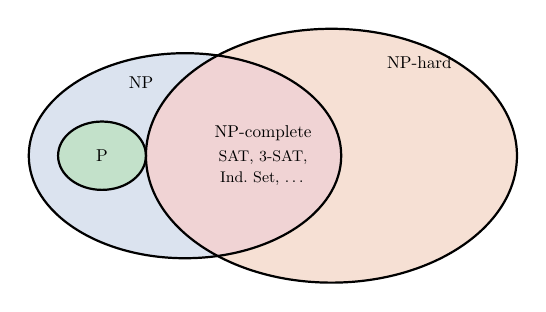
\begin{tikzpicture}[scale=0.62, every node/.append style={transform shape}]
        \fill[mOrange!25] (2.5,0) ellipse (3.8 and 2.6);
        \fill[mLightBlue!20] (-0.5,0) ellipse (3.2 and 2.1);
        \begin{scope}
          \clip (-0.5,0) ellipse (3.2 and 2.1);
          \fill[mRed!25] (2.5,0) ellipse (3.8 and 2.6);
        \end{scope}
        \fill[mGreen!35] (-2.2,0) ellipse (0.9 and 0.7);
        \draw[thick] (2.5,0) ellipse (3.8 and 2.6);
        \draw[thick] (-0.5,0) ellipse (3.2 and 2.1);
        \draw[thick] (-2.2,0) ellipse (0.9 and 0.7);
        \node at (4.3,1.9) {NP-hard};
        \node at (-1.4,1.5) {NP};
        \node[align=center] at (1.1,0) {NP-complete\\[2pt]\small SAT, 3-SAT,\\
          \small Ind.\ Set, \ldots};
        \node at (-2.2,0) {P};
      \end{tikzpicture}\\
      \small The picture if $\mathbf{P} \ne \mathbf{NP}$.
      \end{center}
    \end{column}
  \end{columns}
\end{frame}

\begin{frame}{Why Care?}
  Proving a problem NP-complete is strong evidence that \alert{no}
  polynomial-time algorithm exists: finding one would solve thousands of
  problems that have resisted decades of effort, and settle P vs.\ NP.

  \bigskip
  What to do instead:
  \begin{itemize}
    \item solve \alert{special cases} (trees, small $k$, bounded weights),
    \item settle for an \alert{approximation} with a guarantee,
    \item use \alert{heuristics} that work well in practice,
    \item accept an exponential algorithm that is fast enough for the inputs
          you have (e.g.\ dynamic programming, SAT solvers).
  \end{itemize}
\end{frame}

% =========================================================================
\section{Satisfiability}

\begin{frame}{SAT}
  \begin{itemize}
    \item A \alert{literal} is a variable $x_i$ or its negation $\neg x_i$.
    \item A \alert{clause} is an OR of literals:
          $(\ell_1 \lor \ell_2 \lor \cdots \lor \ell_m)$.
    \item A formula is in \alert{conjunctive normal form} (CNF) if it is an
          AND of clauses.
  \end{itemize}

  \begin{block}{SAT}
    Given a CNF formula $\phi$, is there a true/false assignment to the
    variables that satisfies every clause?
  \end{block}

  \textbf{Example.}
  $\phi = (x_1 \lor \neg x_2) \land (\neg x_1 \lor x_2 \lor x_3)$.
  \pause
  Setting $x_1 = x_2 = \mathrm{T}$, $x_3 = \mathrm{F}$ satisfies both clauses.

  \pause
  \medskip
  SAT $\in \mathbf{NP}$: the certificate is a satisfying assignment; check
  each clause in time linear in the size of $\phi$.
\end{frame}

\begin{frame}{3-SAT}
  \alert{3-SAT} is SAT where every clause has \alert{exactly 3} literals:
  \[
    \phi = (x_1 \lor x_2 \lor \neg x_3) \land
           (\neg x_1 \lor x_2 \lor x_3) \land
           (x_1 \lor \neg x_2 \lor x_3).
  \]

  \begin{itemize}
    \item 3-SAT $\in \mathbf{NP}$, for the same reason as SAT.
    \item 3-SAT is a special case of SAT, so it is no harder.
    \item Its rigid structure makes it a convenient starting point for
          reductions: every clause can become the same small
          \alert{gadget}.
  \end{itemize}

  \bigskip
  \small (2-SAT, with two literals per clause, is in $\mathbf{P}$, via
  strongly connected components!)
\end{frame}

\begin{frame}{The Cook-Levin Theorem}
  \begin{block}{Theorem (Cook 1971; Levin 1973)}
    SAT is NP-complete.
  \end{block}

  \textbf{Idea.} Take any $A \in \mathbf{NP}$ with its polynomial-time
  verifier. Write the verifier's whole computation on input $x$ as a
  polynomial-size CNF formula whose variables are the unknown certificate
  bits and the machine's state at each step. The formula is satisfiable
  $\iff$ some certificate makes the verifier accept. (Proof omitted.)

  \pause
  \bigskip
  \begin{block}{Theorem (Karp 1972)}
    3-SAT is NP-complete.
  \end{block}
  This needs one more reduction, SAT $\le_p$ 3-SAT: split long clauses with
  new variables, e.g.\
  $(\ell_1 \lor \ell_2 \lor \ell_3 \lor \ell_4) \to
   (\ell_1 \lor \ell_2 \lor z) \land (\neg z \lor \ell_3 \lor \ell_4)$.
\end{frame}

\begin{frame}{How to Prove $B$ Is NP-Complete}
  \begin{enumerate}
    \item \textbf{$B \in \mathbf{NP}$}: give a certificate and a
          polynomial-time verifier.
    \item \textbf{$B$ is NP-hard}: pick a known NP-complete problem $A$
          (e.g.\ 3-SAT) and give a reduction $A \le_p B$.
  \end{enumerate}

  \begin{center}
  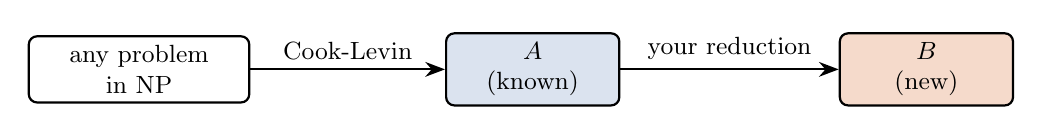
\begin{tikzpicture}
    \node[box, minimum width=28mm] (np) at (0,0) {any problem\\in NP};
    \node[box, fill=mLightBlue!20] (a) at (5,0) {$A$\\(known)};
    \node[box, fill=mOrange!30] (b) at (10,0) {$B$\\(new)};
    \draw[arr] (np) -- node[above, font=\small] {Cook-Levin} (a);
    \draw[arr] (a) -- node[above, font=\small] {your reduction} (b);
  \end{tikzpicture}
  \end{center}

  \pause
  \textbf{Why it works}: reductions compose. If $f$ runs in $O(n^c)$ and $g$
  in $O(n^d)$, then $g \circ f$ runs in $O(n^c + n^{cd})$, and
  \[
    x \in \text{NP problem} \iff f(x) \in A \iff g(f(x)) \in B.
  \]

  \medskip
  \alert{Direction matters}: reduce \emph{from} the known hard problem
  \emph{to} the new one.
\end{frame}

% =========================================================================
\section{3-SAT $\le_p$ Independent Set}

\begin{frame}{Independent Set}
  An \alert{independent set} in $G = (V, E)$ is a set $S \subseteq V$ with no
  edge between any two of its vertices.

  \begin{block}{Independent Set}
    Given $G$ and $k$, does $G$ have an independent set of size $\ge k$?
  \end{block}

  \begin{block}{Theorem}
    Independent Set is NP-complete.
  \end{block}

  \textbf{Step 1: in NP.} Certificate: the set $S$. Check $|S| \ge k$ and
  that no edge has both endpoints in $S$, in $O(n + m)$ time.

  \medskip
  \textbf{Step 2: NP-hard.} Reduce 3-SAT $\le_p$ Independent Set.
\end{frame}

\begin{frame}{The Construction}
  Given a 3-CNF formula $\phi$ with clauses $C_1, \ldots, C_k$:

  \begin{itemize}
    \item \textbf{Clause gadget}: for each clause, three vertices (one per
          literal) joined in a \alert{triangle}. An independent set takes at
          most one vertex per triangle.
    \item \textbf{Conflict edges}: join every pair of vertices in different
          triangles whose literals are \alert{complementary} ($x_r$ and
          $\neg x_r$). An independent set never picks both.
    \item Target size: $k$, the number of clauses.
  \end{itemize}

  \bigskip
  Size: $3k$ vertices, at most $\binom{3k}{2}$ edges. Polynomial time.

  \bigskip
  \textbf{Intuition}: choosing a vertex $=$ choosing which literal makes its
  clause true. Conflict edges keep these choices consistent.
\end{frame}

\begin{frame}{Example}
  $\phi = (x_1 \lor x_2 \lor \neg x_3) \land (\neg x_1 \lor x_2 \lor x_3)
         \land (x_1 \lor \neg x_2 \lor x_3)$, \quad $k = 3$.

  \begin{center}
  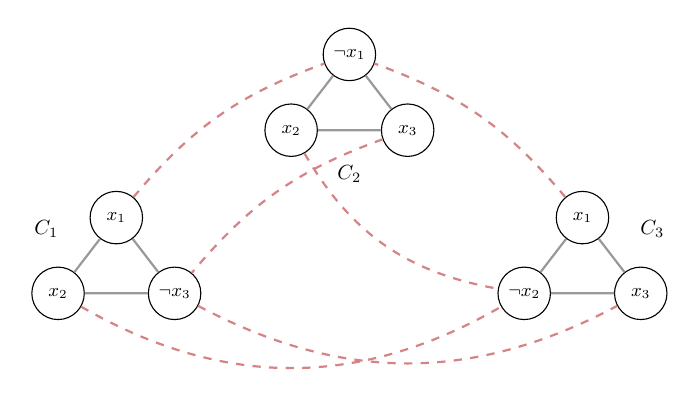
\begin{tikzpicture}[scale=0.74, every node/.append style={transform shape}]
    % C1
    \node[lit, onslide=<2->{pick}] (x1a)  at (0,1.3)  {$x_1$};
    \node[lit] (x2a)  at (-1,0)   {$x_2$};
    \node[lit] (nx3a) at (1,0)    {$\neg x_3$};
    \draw[edg] (x1a) -- (x2a) -- (nx3a) -- (x1a);
    \node at (-1.2,1.1) {$C_1$};
    % C2
    \node[lit] (nx1b) at (4,4.1)  {$\neg x_1$};
    \node[lit, onslide=<2->{pick}] (x2b)  at (3,2.8)  {$x_2$};
    \node[lit] (x3b)  at (5,2.8)  {$x_3$};
    \draw[edg] (nx1b) -- (x2b) -- (x3b) -- (nx1b);
    \node at (4,2.05) {$C_2$};
    % C3
    \node[lit] (x1c)  at (8,1.3)  {$x_1$};
    \node[lit] (nx2c) at (7,0)    {$\neg x_2$};
    \node[lit, onslide=<2->{pick}] (x3c)  at (9,0)    {$x_3$};
    \draw[edg] (x1c) -- (nx2c) -- (x3c) -- (x1c);
    \node at (9.2,1.1) {$C_3$};
    % conflicts
    \draw[conf] (x1a)  to[bend left=15]  (nx1b);
    \draw[conf] (x1c)  to[bend right=15] (nx1b);
    \draw[conf] (x3b)  to[bend right=15] (nx3a);
    \draw[conf] (x2b)  to[bend right=25] (nx2c);
    \draw[conf] (x2a)  to[bend right=30] (nx2c);
    \draw[conf] (nx3a) to[bend right=28] (x3c);
  \end{tikzpicture}
  \end{center}

  \small Solid: clause triangles. \textcolor{mRed}{Dashed}: the six conflict
  edges. \onslide<2->{$x_1 = x_2 = x_3 = \mathrm{T}$ satisfies $\phi$; one
  true literal per clause gives an independent set of size 3 (orange).}
\end{frame}

\begin{frame}{Correctness}
  \textbf{Claim.} $\phi$ is satisfiable $\iff$ $G$ has an independent set of
  size $k$.

  \medskip
  ($\Rightarrow$) Take a satisfying assignment. From each clause pick one
  true literal's vertex; call the set $S$.
  \begin{itemize}
    \item $|S| = k$, one vertex per triangle, so no triangle edge is inside
          $S$.
    \item A conflict edge inside $S$ would mean $x_r$ and $\neg x_r$ are both
          true. Impossible.
  \end{itemize}

  \pause
  ($\Leftarrow$) Let $S$ be an independent set of size $k$.
  \begin{itemize}
    \item Each triangle holds at most one vertex of $S$, and there are $k$
          triangles: exactly one per triangle.
    \item Make every literal in $S$ true. This is consistent: $S$ has no
          conflict edge, so it never contains both $x_r$ and $\neg x_r$.
          Set the remaining variables arbitrarily.
    \item Each clause contains the true literal chosen from its triangle.
          \hfill $\square$
  \end{itemize}
\end{frame}

% =========================================================================
\section{3-SAT $\le_p$ Integer Linear Programming}

\begin{frame}{Integer Linear Programming}
  \begin{block}{ILP Feasibility}
    Given integer coefficients $c_{ji}$ and $d_j$, are there
    \alert{integers} $y_1, \ldots, y_n$ with
    \[
      \sum_{i=1}^{n} c_{ji}\, y_i \ge d_j \quad \text{for every constraint } j?
    \]
  \end{block}

  \begin{block}{Theorem}
    ILP Feasibility is NP-complete.
  \end{block}

  \textbf{Step 1: in NP.} Certificate: the integers $y_i$; check each
  constraint. \small(Subtle point: one must also show that if a solution
  exists, one with polynomially many bits exists. This is true but not
  obvious. For 0/1 variables it is immediate.)

  \normalsize
  \medskip
  \textbf{Step 2: NP-hard.} Reduce 3-SAT $\le_p$ ILP.
\end{frame}

\begin{frame}{The Construction}
  Given $\phi$ with clauses $C_1, \ldots, C_m$ over $x_1, \ldots, x_n$:

  \begin{itemize}
    \item \textbf{Variables}: one integer $y_i$ per $x_i$, with
          $0 \le y_i \le 1$. So $y_i \in \{0, 1\}$: $1$ means true, $0$
          means false.
    \item \textbf{Clause constraints}: for clause $C_j$, let $P_j$ ($N_j$)
          be the indices of its positive (negated) literals:
          \[
            \sum_{i \in P_j} y_i + \sum_{i \in N_j} (1 - y_i) \ge 1.
          \]
          The left side counts the true literals in $C_j$.
  \end{itemize}

  \bigskip
  $n$ variables and $m + 2n$ constraints, built in polynomial time.

  \pause
  \medskip
  \textbf{Correctness}: $y$ satisfies the constraints $\iff$ the assignment
  $x_i = (y_i = 1)$ makes at least one literal true in every clause $\iff$
  it satisfies $\phi$. \hfill $\square$
\end{frame}

\begin{frame}{Examples}
  \begin{columns}[t]
    \begin{column}{0.52\textwidth}
      \textbf{Satisfiable}\\[2pt]
      \small
      $(x_1 \lor x_2 \lor \neg x_3) \land (\neg x_1 \lor x_2 \lor x_3)
       \land (x_1 \lor \neg x_2 \lor x_3)$
      \[
        \begin{aligned}
          y_1 + y_2 + (1 - y_3) &\ge 1 \\
          (1 - y_1) + y_2 + y_3 &\ge 1 \\
          y_1 + (1 - y_2) + y_3 &\ge 1 \\
          0 \le y_i \le 1, \ y_i &\in \mathbb{Z}
        \end{aligned}
      \]
      $y_1 = y_2 = y_3 = 1$: the left sides are $2, 2, 2$. Feasible.
    \end{column}
    \begin{column}{0.45\textwidth}
      \textbf{Unsatisfiable}\\[2pt]
      \small
      $(x_1 \lor x_1 \lor x_1) \land (\neg x_1 \lor \neg x_1 \lor \neg x_1)$
      \[
        \begin{aligned}
          3 y_1 &\ge 1 \\
          3 (1 - y_1) &\ge 1 \\
          0 \le y_1 \le 1, \ y_1 &\in \mathbb{Z}
        \end{aligned}
      \]
      The first forces $y_1 = 1$, the second $y_1 = 0$. Infeasible.
    \end{column}
  \end{columns}

  \bigskip
  \small Without integrality, $y_1 = \tfrac{1}{2}$ would work: plain
  linear programming is in $\mathbf{P}$, and integrality is what makes ILP
  hard.
\end{frame}

% =========================================================================
\begin{frame}{Exercise}
  $\phi = (x_1 \lor x_2 \lor x_3) \land (\neg x_1 \lor \neg x_2 \lor x_3)
         \land (\neg x_3 \lor x_1 \lor x_2)$

  \bigskip
  \begin{enumerate}
    \item Build the Independent Set instance. How many vertices, triangle
          edges, and conflict edges does it have, and what is $k$?
    \item Find a satisfying assignment and the corresponding independent
          set.
    \item Write the ILP instance.
    \item A friend proves Independent Set $\le_p$ SAT. Does that show
          Independent Set is NP-hard?
  \end{enumerate}
\end{frame}

\begin{frame}{Solution}
  \small
  \textbf{(a)} $9$ vertices, $9$ triangle edges, $k = 3$. Conflict edges
  ($6$): $x_1$ in $C_1$ and $C_3$ each with $\neg x_1$ in $C_2$; $x_2$ in
  $C_1$ and $C_3$ each with $\neg x_2$ in $C_2$; $x_3$ in $C_1$ and $C_2$
  each with $\neg x_3$ in $C_3$.

  \medskip
  \textbf{(b)} $x_1 = \mathrm{T}$, $x_2 = \mathrm{F}$, $x_3 = \mathrm{T}$.
  Pick $x_1$ from $C_1$, $\neg x_2$ from $C_2$, $x_1$ from $C_3$. No
  conflict edge joins them.

  \medskip
  \textbf{(c)}
  $y_1 + y_2 + y_3 \ge 1$, \quad $(1 - y_1) + (1 - y_2) + y_3 \ge 1$, \quad
  $(1 - y_3) + y_1 + y_2 \ge 1$, \quad $0 \le y_i \le 1$, $y_i \in
  \mathbb{Z}$.

  \medskip
  \textbf{(d)} No, wrong direction. It shows Independent Set is \emph{no
  harder} than SAT (true for every problem in NP, by Cook-Levin). Hardness
  needs SAT (or 3-SAT) $\le_p$ Independent Set.
\end{frame}

% =========================================================================
\begin{frame}{Summary}
  \begin{itemize}
    \item \textbf{NP-hard}: every NP problem reduces to it.
          \textbf{NP-complete}: NP-hard and in NP.
    \item \textbf{Cook-Levin}: SAT is NP-complete; 3-SAT is too.
    \item To show $B$ is NP-complete: $B \in \mathbf{NP}$, and
          \alert{known NP-complete} $\le_p B$.
    \item 3-SAT $\le_p$ Independent Set: a triangle per clause, conflict
          edges between complementary literals, $k =$ number of clauses.
    \item 3-SAT $\le_p$ ILP: $0/1$ variables, one ``at least one true
          literal'' constraint per clause.
  \end{itemize}
\end{frame}

\end{document}
